

\chapter{Funções de várias variáveis}


\resumo{titulo}{
\begin{itemize}[label=\color{chapterscolor}\textbullet]
    \item Compreender o conceito de função de várias variáveis entendendo que funções de várias variáveis associam um número real a um conjunto de \(n\) valores reais, onde \(n\) é o número de variáveis independentes.
    
    \item Identificar e determinar o domínio da função, domínio de interesse, e suas diferenças. 
    
    \item Reconhecer a imagem da função.
    
    \item Interpretar o gráfico de uma função de duas variáveis e representar graficamente funções de duas variáveis em $\R^3$. 
    
    \item Entender e identificar os conjuntos de nível de uma função.
    
    \item Aplicar os conceitos aprendidos em situações problemas reais. 
\end{itemize}
}




Na economia, muitos fenômenos não podem ser adequadamente descritos por meio de funções com apenas uma variável independente. Por exemplo, a lei da demanda estabelece a relação entre a quantidade de um bem procurado pelo consumidor \(D\) e o preço daquele bem \(p\). Essa relação fundamental sustenta que, à medida que o preço do bem aumenta, a quantidade demandada pelo consumidor diminui, e vice-versa. No entanto, a demanda não depende apenas do preço. De fato, existem outros elementos que podem afetar a quantidade de um bem que os consumidores desejam adquirir, mesmo que o preço permaneça constante, como a renda dos consumidores (\(R\)) e o preço de bens substitutos (\(P_s\)) ou complementares (\(P_c\)). Ou seja, para cada combinação possível de preços e renda \((p, R, P_s, P_c)\), temos uma quantidade demandada do produto \(D(p, R, P_s, P_c)\). 

Essa função \(D\) é importante na economia, pois nos permite entender como a demanda por um produto varia em resposta a mudanças nos preços e na renda dos consumidores. Ela nos ajuda a analisar a sensibilidade da demanda em relação a diferentes fatores e a fazer previsões sobre o comportamento do mercado em diferentes cenários econômicos. 

Assim, diante da complexidade e diversidade dos fatores que influenciam os fenômenos econômicos, torna-se necessário estudar funções que dependem de outras variáveis, que nos permitem analisar e modelar situações mais realistas, em que múltiplos fatores interagem para determinar um resultado específico. 



\begin{definition}{Função real de várias variáveis reais}{def_funcao}
Uma \textit{função real de várias variáveis reais} é uma função matemática \( f \) que associa um número real (\textit{variável dependente}) a cada combinação ordenada de valores reais (variáveis independentes) pertencentes a um certo conjunto chamado de \textit{domínio}\index{função!domínio de uma}\index{domínio de uma função} de $f$. 
\myrule{definitioncolor!140}
Denotaremos o domínio de $f$ por $\Dom(f)$. A \textit{imagem}\index{função!imagem de uma}\index{imagem de uma função} de $f$ é o conjunto 
$$\Img(f)%=\left\{y\in \R ;~ y= f(\Point{x}),~\Point{x}\in D\right\}
=\left\{f(\Point{x});~\Point{x}\in D\right\}\subset\R.$$
\end{definition}
Em outras palavras, se \( \Point{x} = (x_1, x_2, \ldots, x_m)\in\R^n \) é um elemento de \( \Dom(f) \), então \( f(\Point{x}) \) é um número real pertence ao intervalo $\Img(f)$. Escrevemos formalmente
\[ f: \Dom(f) \subset \mathbb{R}^n \rightarrow \mathbb{R}. \]

Por exemplo, a função \(f(x,y) = x^2 + y^2\) é definida nas variáveis \(x\) e \(y\), com um domínio que abrange todo o plano \(\mathbb{R}^2\), e sua imagem consiste em todos os valores não negativos \([0, \infty)\). Em contrapartida, a função \(g(x,y) = \sqrt{1-x^2-y^2}\) tem um domínio limitado à bola fechada centrada na origem e com raio 1, denotada por \(\overline{B(0,1)}\), e sua imagem também é o intervalo \([0, \infty)\).

Por outro lado, nem sempre é necessário estudar uma função em todo o seu domínio de definição, mas sim em um subconjunto \(D \subset \Dom(f)\). Nesse caso, representamos a função como \(f: D \to \mathbb{R}\), ou também como \(f|_D\), que é lido como \textit{$f$ restrita ao subconjunto $D$}. Dizemos que $D$ é o \textit{domínio de interesse}\index{domínio!de interesse de uma função}\index{função!domínio de interesse de uma} de $f$. 

Para exemplificar este fato consideremos a função
$$U(x,y)=x^{\frac{1}{2}}y^{\frac{1}{2}}.$$
Temos que 
$$\Dom(f)=\left\{(x,y)\in\R^2; ~ x\geq 0,~y\geq 0\right\},$$
pois a função \textit{raiz quadrada} não está definida sobre os números negativos. Por outro lado, suponha que essa função modela as preferências de um consumidor em relação a diferentes quantidades de dois bens, $X$ e $Y$, que ele pode consumir. Nesse contexto tal consumidor deve ter um orçamento, digamos, R\$1000. Supondo que o valor unitário do produto $X$ é R\$ 50 e o de $Y$ é R\$ 30, temos a seguinte restrição orçamentária: 
$$50x+30y\leq 1000,$$
e a função $U$ tem interesse prático restrita ao subconjunto
$$D=\left\{(x,y)\in \R^2;~x\geq 0,~y\geq0,~50x+30y\leq 1000 \right\}.$$
Ou seja, o conjunto de interesse neste caso não é o domínio de $f$ e sim o conjunto do Exemplo \ref{modelo1}. 



A função $U$ anterior é chamada de Cobb-Douglass, em homenagem a dois economistas americanos, Charles W. Cobb e Paul H. Douglas que a introduziram em 1928, em um artigo intitulado ``A Theory of Production''. No exemplo apresentado $U$ descreve como o consumidor atribui valor ou utilidade a cada combinação dos bens $X$ e $Y$, isto é, $U$ é um exemplo de uma \textit{função de utilidade}\index{função!de utilidade}.  

A \textit{grosso modo}, uma função de utilidade atribui um valor numérico (ou utilidade) a cada possível cesta de consumo, ou seja, a cada combinação de $n$ bens ou serviços que o consumidor pode escolher. Essa utilidade reflete o grau de satisfação ou felicidade que o consumidor obtém de cada cesta de consumo. Vejamos alguns exemplos de função de utilidade. 

\index{função!de utilidade}
\begin{example}{Função de utilidade para $n$ bens}{exem:funcao_utilidade}
Dado \(n\) bens de consumo, representamos por \(x_1, x_2, \ldots, x_n\) suas respectivas quantidades. A função de utilidade é denotada por \(U\) e atribui a cada combinação específica de quantidades dos bens, \((x_1, x_2, \ldots, x_n)\), um número real \(U(x_1, x_2, \ldots, x_n)\) que reflete a utilidade total do consumidor com essa cesta de consumo. %Em outras palavras, a função de utilidade \(U\) mapeia as quantidades dos bens \(x\) em um valor numérico que expressa a satisfação ou preferência do consumidor em relação àquela combinação específica de consumo. 

\myrule{examplescolor}
\textbf{Utilidade Cobb-Douglas:}\smallskip
\index{função!de utilidade!de Cobb-Douglas}

A função de utilidade Cobb-Douglas é dada por: 
\[ U(x_1, x_2, \ldots, x_n) = A \cdot x_1^{\alpha_1} \cdot x_2^{\alpha_2} \cdot \ldots \cdot x_n^{\alpha_n}, \]
onde 
%\( A \) é uma constante positiva que representa a utilidade total quando todas as quantidades dos bens são iguais a 1 e 
\( \alpha_1, \alpha_2, \ldots, \alpha_n \) são os coeficientes que medem as elasticidades de produção ou preferências de cada bem ou fator de produção (tais coeficientes devem ser estritamente positivos e a soma deles deve ser menor que 1 para garantir a substituibilidade entre os bens). 
%A função de utilidade Cobb-Douglas também é um exemplo clássico amplamente utilizado na economia. Ela é dada por \(U(x, y) = x^{\alpha} \cdot y^{\beta}\), onde \(x\) e \(y\) são as quantidades de dois bens, e \(\alpha\) e \(\beta\) são coeficientes positivos que medem a importância relativa de cada bem na utilidade total. A função de utilidade Cobb-Douglas apresenta elasticidades de substituição constantes e é amplamente usada para analisar a demanda do consumidor e a alocação de recursos.


%\myrule{examplescolor}
%\textbf{Utilidade Logarítmica:}\index{função!de utilidade!logarítmica}\smallskip
%A função de utilidade logarítmica é uma versão da função de utilidade anterior. Ela é dada por \(U(x, y) = \alpha \ln(x) + \beta \ln(y)\), onde \(x\) e \(y\) são as quantidades de dois bens, e \(\alpha\) e \(\beta\) são coeficientes positivos. Essa função é comumente usada para representar a utilidade de bens que têm retornos marginais decrescentes, como no caso de consumo de alimentos ou lazer.

\myrule{examplescolor}

\textbf{Utilidade Quadrática:}\index{função!de utilidade!quadrática}\smallskip

De forma mais geral, a função de utilidade quadrática é dada por 
\[ U(x_1, x_2, \ldots, x_n) = a_1 x_1^2 + a_2 x_2^2 + \ldots + a_n x_n^2, \]
onde \( a_1, a_2, \ldots, a_n \) são coeficientes positivos que medem a importância relativa ou o peso de cada bem ou fator de produção na função de utilidade ou de produção. Nesse caso, a utilidade total ou a quantidade produzida é uma soma ponderada dos quadrados das quantidades dos \( n \) bens ou fatores de produção. Cada coeficiente \( a_i \) representa a importância ou a utilidade marginal de cada bem ou fator de produção. Valores maiores para \( a_i \) indicam que o consumidor valoriza mais a quantidade do bem ou fator \( x_i \), enquanto valores menores implicam em uma valoração menor.

%A função de utilidade quadrática é outro exemplo comum, especialmente em análises de bem-estar econômico. Ela é dada por \(U(x, y) = ax^2 + by^2\), onde \(x\) e \(y\) são as quantidades de dois bens, e \(a\) e \(b\) são coeficientes positivos. Essa função é utilizada para analisar casos em que o consumidor valoriza intensamente grandes quantidades de um bem específico.


\end{example}

%%%

\begin{comment}
Um exemplo de função de várias variáveis muito significativo na economia é a função de produção Cobb-Douglas, amplamente utilizada na teoria econômica para modelar a relação entre os fatores de produção e a quantidade produzida de um bem ou serviço. Essa função recebe esse nome em homenagem aos economistas Charles Cobb e Paul Douglas, que a introduziram em 1928.

A função de produção Cobb-Douglas é dada pela seguinte equação:
\[ Q = A \cdot L^{\alpha} \cdot K^{\beta},\]
onde 
\begin{itemize}
  \item \( Q \) é a quantidade produzida do bem ou serviço;
  \item \( L \) é a quantidade de trabalho utilizado na produção;
  \item \( K \) é a quantidade de capital utilizado na produção;
  \item \( A \) é uma constante positiva que representa a tecnologia ou a eficiência total dos fatores de produção;
  \item \( \alpha \) e \( \beta \) são os parâmetros que medem as elasticidades de produção do trabalho e do capital, respectivamente.
\end{itemize}


Essa função de produção é muito utilizada para analisar a produtividade e eficiência das empresas e indústrias, bem como para entender o impacto das mudanças nos fatores de produção na quantidade produzida. Além disso, ela é frequentemente usada para estudar a alocação ótima de recursos e para fazer previsões sobre o crescimento econômico.

A função de produção Cobb-Douglas é um exemplo significativo de como as funções matemáticas são aplicadas na economia para modelar fenômenos complexos e fornecer insights importantes para a tomada de decisões econômicas.
\end{comment}

\begin{exercise}{}{}
Suponha que a demanda por refrigeradores em uma determinada região depende dos seguintes fatores:
\begin{itemize}[label=\color{green!140}\textbullet]
\item \(p\): o preço do refrigerador,
\item \(R\): a renda dos consumidores,
\item \(P_s\): o preço de bens substitutos,
\item \(P_c\): o preço de bens complementares.
\end{itemize}

\begin{enumerate}[label=\color{green!140}(\alph*)]
\item Crie uma função \textit{hipotética} que modele a quantidade demandada considerando os seguintes comportamentos:
\begin{itemize}[label=\color{green!140}\textbullet]
\item Quando o preço do refrigerador diminui, a quantidade demandada aumenta, ou seja, há uma relação inversamente proporcional entre o preço e a quantidade demandada.
\item Um aumento na renda dos consumidores tende a aumentar a quantidade demandada de refrigeradores, ou seja, a quantidade demandada está positivamente relacionada à renda dos consumidores.
\item Se os bens substitutos, como freezers ou outros eletrodomésticos de refrigeração, tornarem-se mais caros, a demanda por refrigeradores pode diminuir, indicando que a mesma está inversamente relacionada ao preço dos bens substitutos. 
\item Se os bens complementares, como utensílios para uso em conjunto com o refrigerador, ficarem mais caros, isso pode aumentar a demanda por refrigeradores, o que sugere que está positivamente relacionada ao preço de bens complementares.
\end{itemize}

\item Determine o domínio da sua função.

\item Determine o conjunto sobre o qual sua função reflete a realidade do problema. 

\end{enumerate}

\end{exercise}



\section{Gráfico de uma função de várias variáveis}


\begin{definition}{Gráfico de uma função de várias variáveis}{def:grafico}
O \textit{gráfico}\index{gráfico!de uma função de várias variáveis}\index{função!gráfico de uma} de uma função $f$ definida sobre um conjunto $D\in\R^n$ é o conjunto no espaço \(n+1\)-dimensional dado por 
\begin{align*}
\Gr(f)
=&\left\{(x_1, x_2, \ldots, x_n, f(x_1, x_2, \ldots, x_n))\in\R^{n+1};~(x_1, x_2, \ldots, x_n)\in D \right\}.
%=\Big\{(x_1, x_2, \ldots, x_n, y) \in\R^{n+1};~y=f(x_1, x_2, \ldots, x_n)
%\\&\ \ \ 
%\mbox{ e }(x_1, x_2, \ldots, x_n)\in D \Big\}.
\end{align*}

\end{definition}

Em outras palavras, o gráfico da função consiste em uma coleção de pontos no espaço \(n+1\)-dimensional, onde \(n\) dimensões representam as coordenadas das variáveis independentes e a dimensão adicional ou \textit{altura} representa o valor da função para cada combinação de valores das variáveis independentes.


\begin{example}{}{exem:grafico}

\begin{itemize}[label=\color{examplescolor}\textbullet]
\item O gráfico da função $f(x,y)=30-\frac{x}{10}-\frac{y}{2}$ é o conjunto 
$$\left\{(x,y,z)\in\R^3;~z= 30-\frac{x}{10}-\frac{y}{2}\right\}\subset\R^3,$$
ou seja, o plano de equação $10x+50y+100z=3000$. 
Observe que no Exemplo \ref{exem:modelo2} já vimos o gráfico da função $f$ restrita a um certo domínio de interesse. 
\begin{center}

\tdplotsetmaincoords{70}{110} % Adjust the view angles (azimuth, elevation)

\begin{tikzpicture}[scale=1.5,tdplot_main_coords]
    % Eixos coordenados
    \draw[-latex] (0,0,0) -- (3,0,0) node[below] {$x$};
    \draw[-latex] (0,0,0) -- (0,3,0) node[right] {$y$};
    \draw[-latex] (0,0,0) -- (0,0,3) node[above] {$z$};
    
    % Pontos que definem o plano
    \coordinate (A) at (2,0,0);
    \coordinate (B) at (0,2,0);
    \coordinate (C) at (0,0,2.5);

\draw[dashed,gray] (1/2,0,0) -- (1/2,1/2,0)
node[right]{\small$(x,y)$} -- (0,1/2,0);
\draw[dashed,gray] (1/2,1/2,0) -- (1/2,1/2,2) ;     

    
    % Desenho do plano
    \draw[blue!140,fill=blue!10,opacity=0.75] (A) -- (B) -- (C) -- cycle;
    
    \filldraw[red!150] (1/2,1/2,2) circle (1pt) node[right]{\small$\left(x,y,\frac{3000-10x-50y}{100}\right)$};
    
    % Rótulos dos pontos
    \node[left] at (A) {\footnotesize $300$};
    \node[above] at (B) {\footnotesize $50$};
    \node[left] at (C) {\footnotesize $100$};
\end{tikzpicture}
\end{center}



De forma geral, todos os planos são gráficos de funções que dependem de $x$ e $y$, pois $z$ pode ser escrita explicitamente em função de $x$ e de $z$. 



\item O gráfico da função $g(x,y)=x^2+y^2$ é o paraboloide  
$$\left\{(x,y,z);~z=x^2+y^2\right\}.$$
\begin{center}
\tdplotsetmaincoords{70}{110} % Adjust the view angles (azimuth, elevation)
    \begin{tikzpicture}[tdplot_main_coords,scale=2.0]
		\pgfmathsetmacro{\tini}{0.5*pi}
		\pgfmathsetmacro{\tfin}{1.85*pi}
		\pgfmathsetmacro{\tend}{2.5*pi}
		% Node indicating the equation of the circumference
%		\draw[white] (1.35,0,0) -- (0,1.35,0) node [red,below,midway,sloped] {$x^2 + y^2 = 1$};
		%%% Coordinate axis
		\draw[-latex] (0,0,0) -- (1.5,0,0) node [below left] {$x$};
		\draw[dashed] (0,0,0) -- (-1.25,0,0);
		\draw[-latex] (0,0,0) -- (0,1.5,0) node [right] {$y$};
		\draw[dashed] (0,0,0) -- (0,-1.25,0);
		% The region of integration
		%\fill[yellow,opacity=0.35] plot[domain=0:6.2832,smooth,variable=\t] ({cos(\t r)},{sin(\t r)},{0.0});
		%\draw[red,thick] plot[domain=0:6.2832,smooth,variable=\t] ({cos(\t r)},{sin(\t r)},{0.0});
		% The curves slicing the surface
\draw[blue!140] plot[domain=-1:1,smooth,variable=\t] ({\t},0,{\t*\t}); 
		%\draw[blue!140,opacity=0.5] plot[domain=-1:1,smooth,variable=\t] (0,{\t},{\t*\t}); 
		% El paraboloid (for z = constant)
		\foreach \altura in {0.0125,0.025,...,1.0}{
			\pgfmathparse{sqrt(\altura)}
			\pgfmathsetmacro{\radio}{\pgfmathresult}
			\draw[blue!50,opacity=0.5] plot[domain=\tini:\tfin,smooth,variable=\t] ({\radio*cos(\t r)},{\radio*sin(\t r)},{\altura}); 
		}
		% Circunference bounding the surface (above, first part)
%		\draw[blue,opacity=0.75] plot[domain=pi:1.75*pi,smooth,variable=\t] ({cos(\t r)},{sin(\t r)},{1.0}); 
		% last part of the z axis
		\draw[-latex] (0,0,0) -- (0,0,1.75) node [above] {$z$};	
		\foreach \altura in {0.0125,0.025,...,1.0}{
			\pgfmathparse{sqrt(\altura)}
			\pgfmathsetmacro{\radio}{\pgfmathresult}
			\draw[blue!50,opacity=0.5] plot[domain=\tfin:\tend,smooth,variable=\t] ({\radio*cos(\t r)},{\radio*sin(\t r)},{\altura}); 
		}
		% Circunference bounding the surface (above, last part)
%		\draw[blue,opacity=0.75] plot[domain=-0.25*pi:pi,smooth,variable=\t] ({cos(\t r)},{sin(\t r)},{1.0}); 

    
\draw[dashed,gray!50] (0.5,-0.5,0) -- (0.5,-0.5,{2*(0.5)^2});
\draw[dashed,gray!50] (0.5,0,0) -- (0.5,-0.5,0)--(0,-0.5,0);

\filldraw[red!150] (0.5,-0.5,{sqrt(1-2*(0.5)^2)}) circle (1pt) node[left]{\small$\left(x,y,x^2+y^2\right)$};


%\node[above right] at (-1,0.5,0.75) {$x_3 = x_1^2 + x_2^2$};
  
	\end{tikzpicture}
\end{center}





\item O gráfico da função $h(x,y)=\sqrt{1-x^2-y^2}$ é a semiesfera superior:
$$\left\{(x,y,z)\in\R^3;~z=\sqrt{1-x^2-y^2},~x^2+y^2\leq 1\right\}.$$
Observe que neste conjunto temos a restrição $x^2+y^2\leq 1$ que está indicando que estamos considerando apenas os pontos $(x,y)$ que estão no domínio de $f$. 
\begin{center}
\tdplotsetmaincoords{70}{110} % Adjust the view angles (azimuth, elevation)
    \begin{tikzpicture}[tdplot_main_coords,scale=2.0]
		\pgfmathsetmacro{\tini}{0.5*pi}
		\pgfmathsetmacro{\tfin}{1.85*pi}
		\pgfmathsetmacro{\tend}{2.5*pi}
		% Node indicating the equation of the circumference
%		\draw[white] (1.35,0,0) -- (0,1.35,0) node [red,below,midway,sloped] {$x^2 + y^2 = 1$};
		%%% Coordinate axis
		\draw[-latex] (0,0,0) -- (1.5,0,0) node [below left] {$x$};
		\draw[dashed] (0,0,0) -- (-1.25,0,0);
		\draw[-latex] (0,0,0) -- (0,1.5,0) node [right] {$y$};
		\draw[dashed] (0,0,0) -- (0,-1.25,0);
		% The region of integration
		%\fill[yellow,opacity=0.35] plot[domain=0:6.2832,smooth,variable=\t] ({cos(\t r)},{sin(\t r)},{0.0});
		%\draw[red,thick] plot[domain=0:6.2832,smooth,variable=\t] ({cos(\t r)},{sin(\t r)},{0.0});
		% The curves slicing the surface
	%\draw[blue!140] plot[domain=-1:1,smooth,variable=\t] ({\t},0,{\t*\t}); 
		%\draw[blue!140,opacity=0.5] plot[domain=-1:1,smooth,variable=\t] (0,{\t},{\t*\t}); 
		% El paraboloid (for z = constant)
		\foreach \altura in {0.0125,0.025,...,1.0}{
			\pgfmathparse{sqrt(1-\altura^2)}
			\pgfmathsetmacro{\radio}{\pgfmathresult}
			\draw[blue!50,opacity=0.5] plot[domain=\tini:\tfin,smooth,variable=\t] ({\radio*cos(\t r)},{\radio*sin(\t r)},{\altura}); 
		}
		% Circunference bounding the surface (above, first part)
%		\draw[blue,opacity=0.75] plot[domain=pi:1.75*pi,smooth,variable=\t] ({cos(\t r)},{sin(\t r)},{1.0}); 
		% last part of the z axis
		\draw[-latex] (0,0,0) -- (0,0,1.75) node [above] {$z$};	
		\foreach \altura in {0.0125,0.025,...,1.0}{
			\pgfmathparse{sqrt(1-\altura^2)}
			\pgfmathsetmacro{\radio}{\pgfmathresult}
			\draw[blue!50,opacity=0.5] plot[domain=\tfin:\tend,smooth,variable=\t] ({\radio*cos(\t r)},{\radio*sin(\t r)},{\altura}); 
		}
		% Circunference bounding the surface (above, last part)
%		\draw[blue,opacity=0.75] plot[domain=-0.25*pi:pi,smooth,variable=\t] ({cos(\t r)},{sin(\t r)},{1.0}); 

    
\draw[dashed,gray!50] (0.5,-0.5,0) -- (0.5,-0.5,{2*(0.5)^2});
\draw[dashed,gray!50] (0.5,0,0) -- (0.5,-0.5,0)--(0,-0.5,0);

\filldraw[red!150] (0.5,-0.5,{sqrt(1-2*(0.5)^2)}) circle (1pt) node[left]{\small$\left(x,y,\sqrt{1-x^2+y^2}\right)$};


%\node[above right] at (-1,0.5,0.75) {$x_3 = x_1^2 + x_2^2$};
  
	\end{tikzpicture}
\end{center}


\item O gráfico da função $i(x,y)=\sqrt{x^2+y^2}$ é o conjunto
$$\Gr(i)\left\{(x,y,z)\in\R^3;~z=\sqrt{x^2+y^2}\right\},$$
que é a parte superior de um cone.
\begin{center}
\tdplotsetmaincoords{70}{110} % Adjust the view angles (azimuth, elevation)

    \begin{tikzpicture}[tdplot_main_coords,scale=2.0]
		\pgfmathsetmacro{\tini}{0.5*pi}
		\pgfmathsetmacro{\tfin}{1.85*pi}
		\pgfmathsetmacro{\tend}{2.5*pi}
		% Node indicating the equation of the circumference
%\draw[white] (1.35,0,0) -- (0,1.35,0) node [red,below,midway,sloped] {$x^2 + y^2 = 1$};
		%%% Coordinate axis
\draw[-latex] (0,0,0) -- (1.5,0,0) node [below left] {$x$};
\draw[dashed] (0,0,0) -- (-1.25,0,0);
\draw[-latex] (0,0,0) -- (0,1.5,0) node [right] {$y$};
\draw[dashed] (0,0,0) -- (0,-1.25,0);
		% The region of integration
		%\fill[yellow,opacity=0.35] plot[domain=0:6.2832,smooth,variable=\t] ({cos(\t r)},{sin(\t r)},{0.0});
		%\draw[red,thick] plot[domain=0:6.2832,smooth,variable=\t] ({cos(\t r)},{sin(\t r)},{0.0});
		% The curves slicing the surface
	%\draw[blue!140] plot[domain=-1:1,smooth,variable=\t] ({\t},0,{\t*\t}); 
		%\draw[blue!140,opacity=0.5] plot[domain=-1:1,smooth,variable=\t] (0,{\t},{\t*\t}); 
		% El paraboloid (for z = constant)
		\foreach \altura in {0.0125,0.025,...,1.0}{
			\pgfmathparse{\altura}
			\pgfmathsetmacro{\radio}{\pgfmathresult}
			\draw[blue!50,opacity=0.5] plot[domain=\tini:\tfin,smooth,variable=\t] ({\radio*cos(\t r)},{\radio*sin(\t r)},{\altura}); 
		}
		% Circunference bounding the surface (above, first part)
%		\draw[blue,opacity=0.75] plot[domain=pi:1.75*pi,smooth,variable=\t] ({cos(\t r)},{sin(\t r)},{1.0}); 
		% last part of the z axis
		\draw[-latex] (0,0,0) -- (0,0,1.75) node [above] {$z$};	
		\foreach \altura in {0.0125,0.025,...,1.0}{
			\pgfmathparse{\altura}
			\pgfmathsetmacro{\radio}{\pgfmathresult}
			\draw[blue!50,opacity=0.5] plot[domain=\tfin:\tend,smooth,variable=\t] ({\radio*cos(\t r)},{\radio*sin(\t r)},{\altura}); 
		}
		% Circunference bounding the surface (above, last part)
%		\draw[blue,opacity=0.75] plot[domain=-0.25*pi:pi,smooth,variable=\t] ({cos(\t r)},{sin(\t r)},{1.0}); 

    
\draw[dashed,gray!50] (0.5,-0.5,0) -- (0.5,-0.5,{2*(0.5)^2});
\draw[dashed,gray!50] (0.5,0,0) -- (0.5,-0.5,0)--(0,-0.5,0);


%\filldraw[red!150] (0.5,-0.5,{sqrt(2*(0.5)^2)}) circle (1pt) node[left]{\small$\left(x,y,\sqrt{x^2+y^2}\right)$};

\shade[ball color=red!100!red!10!white,opacity=1] (0.5,-0.5,{sqrt(2*(0.5)^2)}) circle (1pt);


%\node[above right] at (-1,0.5,0.75) {$x_3 = x_1^2 + x_2^2$};
  
	\end{tikzpicture}
\end{center}



\end{itemize}

\myrule{examplescolor}
    


\begin{itemize}[label=\color{examplescolor}\textbullet]

\item Por outro lado, as esferas não são gráficos pois toda reta vertical a intersecta em dois pontos, o que viola o conceito de função em matemática, já que toda função associa apenas um valor a cada ponto o domínio. De fato, considerando o exemplo modelo da esfera de raio 1, para cada $(x,y)\in B(O,1)\subset \R^2$, os pontos $(x,y,\sqrt{1-x^2-y^2})$ e $(x,y,-\sqrt{1-x^2-y^2})$ estão sobre a esfera. 

\item Da mesma forma, o cone de equação $z^2 = x^2 + y^2$ não é um gráfico. 

\end{itemize}


\end{example}




\section{Conjuntos de nível e mapas de contorno}

\begin{definition}{}{}
Dada uma função \( f: D \subset \mathbb{R}^n \rightarrow \mathbb{R} \), o \textit{conjunto de nível} \( N_c \) para um número real \( c \) é dado por:
\[ N_c = \{(x_1, x_2, \ldots, x_n) \in D \mid f(x_1, x_2, \ldots, x_n) = c \}.\]
\end{definition}

Em outras palavras, o conjunto de nível \( N_c \) é o conjunto de todos os pontos no domínio da função cujo valor é igual a \( c \). 

Um \textit{mapa de contorno}\index{mapa de contorno} é uma representação gráfica que mostra as curvas de nível de uma função de duas variáveis, conectando pontos onde a função tem o mesmo valor constante $c$. A visualização de um mapa de contorno é muito útil para entender as características da função em análise, como pontos críticos (máximos, mínimos e pontos de sela), regiões onde a função cresce ou decresce, e a forma geral da superfície criada pela função no plano.




\subsection{Funções de duas variáveis: Curvas de nível}


Observe agora que se um ponto $(x, y)$ pertence ao domínio de uma função $f$, a ideia do gráfico é que esse ponto é transladado até uma altura $z = f(x, y)$ no espaço tridimensional $\mathbb{R}^3$. Ao intersecionarmos esse gráfico com um plano horizontal $z = c$, obtemos todos os pontos do gráfico que estão na altura $c$. Em outras palavras, isso representa o conjunto:
\[
\{(x, y, z) \in \mathbb{R}^3;~ z = f(x, y) = c;~ (x, y) \in \text{Dom}(f)\}.
\]
Podemos concluir, então, que as curvas de nível são a projeção dessa interseção no plano $xy$.

Essa forma de visualizar as curvas de nível como interseções com planos paralelos ao plano $xy$ pode ajudar a obter uma melhor compreensão do comportamento geral de uma função de duas variáveis por meio da análise de um mapa de contorno.






\begin{example}{}{}
Consideremos a função \(f(x,y) = x^2 + y^2\). Vamos descrever de forma geral suas curvas de nível. Primeiro vejamos que o domínio da função é $\R^2$ e a imagem é $[0,\infty)$. Agora, vamos analisar o comportamento de \(f(x,y)\):
\begin{itemize}[label=\color{examplescolor}\textbullet]

\item $c<0$: como $f$ é não negativa -- pois seu valor é a soma de dois quadrados, então $N_c=\emptyset$.

\item $c=0$: o único ponto onde \(f(x,y) = 0\) é a origem \((0,0)\). Logo $N_0=\{(0,0)\}$. 


\item $c>0$: neste caso a condição $f(x,y)=c>0$ se traduz em $x^2+y^2=c$. Ou seja, a forma das curvas de nível de $f$ são círculos  concêntricos com centros na origem e cujos raios são a raiz dos valores da função:
$$N_c=\{(x,y)\in D; x^2+y^2=c\}$$
\end{itemize}

Na figura a seguir ilustramos o gráfico da função, a interseção desse gráfico com planos em diferentes \textit{níveis} de altura, e o respectivo mapa de contorno 
\begin{center}
\tdplotsetmaincoords{70}{110} % Adjust the view angles (azimuth, elevation)
    \begin{tikzpicture}[tdplot_main_coords,scale=1.75]
		\pgfmathsetmacro{\tini}{0.5*pi}
		\pgfmathsetmacro{\tfin}{1.85*pi}
		\pgfmathsetmacro{\tend}{2.5*pi}
		% Node indicating the equation of the circumference
		%%% Coordinate axis
		\draw[-latex] (0,0,0) -- (2.5,0,0) node [below left] {$x$};
		\draw[dashed] (0,0,0) -- (-2,0,0);
		\draw[-latex] (0,0,0) -- (0,2.5,0) node [right] {$y$};
		\draw[dashed] (0,0,0) -- (0,-2,0);
		% The region of integration

%mapa de contorno
\foreach \altura in {0.25,0.5,...,1.75}{
			\pgfmathparse{sqrt(\altura)}
			\pgfmathsetmacro{\radio}{\pgfmathresult}
			\draw[red!140] plot[domain=0:2*pi,smooth,variable=\t] ({\radio*cos(\t r)},{\radio*sin(\t r)},{0}); 
		}




% paraboloid (for z = constant)
\foreach \altura in {0.0125,0.025,...,2.0}{
			\pgfmathparse{sqrt(\altura)}
			\pgfmathsetmacro{\radio}{\pgfmathresult}
			\draw[blue!50,opacity=0.5] plot[domain=\tini:\tfin,smooth,variable=\t] ({\radio*cos(\t r)},{\radio*sin(\t r)},{\altura}); 
		}

%parte de atrás das curvas de nível
\foreach \altura in {0.25,0.5,...,1.75}{
			\pgfmathparse{sqrt(\altura)}
			\pgfmathsetmacro{\radio}{\pgfmathresult}
			\draw[red!140] plot[domain=\tini:\tfin,smooth,variable=\t] ({\radio*cos(\t r)},{\radio*sin(\t r)},{\altura}); 
		}


\draw[-latex] (0,0,0) -- (0,0,2.75) node [above] {$z$};	



\foreach \altura in {0.0125,0.025,...,2.0}{
			\pgfmathparse{sqrt(\altura)}
			\pgfmathsetmacro{\radio}{\pgfmathresult}
			\draw[blue!50,opacity=0.5] plot[domain=\tfin:\tend,smooth,variable=\t] ({\radio*cos(\t r)},{\radio*sin(\t r)},{\altura}); 
		}

%parte de atrás das curvas de nível
\foreach \altura in {0.25,0.5,...,1.75}{
			\pgfmathparse{sqrt(\altura)}
			\pgfmathsetmacro{\radio}{\pgfmathresult}
			\draw[red!140] plot[domain=\tfin:\tend,smooth,variable=\t] ({\radio*cos(\t r)},{\radio*sin(\t r)},{\altura});
		}

\end{tikzpicture}
\end{center}


Observe na figura como a interseção dos planos horizontais abaixo do plano $xy$ com o paraboloide (que é o gráfico de $f$) é vazia, com o plano de equação $z=0$ é a origem e com planos horizontais acima do plano $xy$ são círculos. 

\end{example}



\newpage

\begin{example}{}{}
Seja \(f(x,y) = \sqrt{x^2 + y^2}\). Primeiro vejamos que o domínio da função é $\R^2$ e a imagem é $[0,\infty)$. Agora, vamos analisar o comportamento de \(f(x,y)\):
\begin{itemize}[label=\color{examplescolor}\textbullet]

\item $c<0$: como $f$ é não negativa -- a raiz quadrada é sempre positiva, então $N_c=\emptyset$.

\item $c=0$: o único ponto onde \(f(x,y) = 0\) é a origem \((0,0)\). Logo $N_0=\{(0,0)\}$. 


\item $c>0$: neste caso a condição $f(x,y)=c>0$ se traduz em $x^2+y^2=c^2$. Ou seja, a forma das curvas de nível de $f$ são círculos  concêntricos com centros na origem e cujos raios são exatamente os valores da função:
$$N_c=\{(x,y)\in D; x^2+y^2=c^2\}$$
\end{itemize}

Na figura a seguir ilustramos o gráfico da função, a interseção desse gráfico com planos em diferentes \textit{níveis} de altura, e o respectivo mapa de contorno 
\begin{center}
\tdplotsetmaincoords{70}{110} % Adjust the view angles (azimuth, elevation)
    \begin{tikzpicture}[tdplot_main_coords,scale=1.75]
		\pgfmathsetmacro{\tini}{0.5*pi}
		\pgfmathsetmacro{\tfin}{1.85*pi}
		\pgfmathsetmacro{\tend}{2.5*pi}
		% Node indicating the equation of the circumference
		%%% Coordinate axis
		\draw[-latex] (0,0,0) -- (2.5,0,0) node [below left] {$x$};
		\draw[dashed] (0,0,0) -- (-2,0,0);
		\draw[-latex] (0,0,0) -- (0,2.5,0) node [right] {$y$};
		\draw[dashed] (0,0,0) -- (0,-2,0);
		% The region of integration

\foreach \altura in {0.25,0.5,...,1.75}{
			\pgfmathparse{\altura}
			\pgfmathsetmacro{\radio}{\pgfmathresult}
			\draw[red!140] plot[domain=0:2*pi,smooth,variable=\t] ({\radio*cos(\t r)},{\radio*sin(\t r)},{0}); 
		}




% paraboloid (for z = constant)
\foreach \altura in {0.0125,0.025,...,2.0}{
			\pgfmathparse{\altura}
			\pgfmathsetmacro{\radio}{\pgfmathresult}
			\draw[blue!50,opacity=0.5] plot[domain=\tini:\tfin,smooth,variable=\t] ({\radio*cos(\t r)},{\radio*sin(\t r)},{\altura}); 
		}

%parte de atrás das curvas de nível
\foreach \altura in {0.25,0.5,...,1.75}{
			\pgfmathparse{\altura}
			\pgfmathsetmacro{\radio}{\pgfmathresult}
			\draw[red!140] plot[domain=\tini:\tfin,smooth,variable=\t] ({\radio*cos(\t r)},{\radio*sin(\t r)},{\altura}); 
		}


\draw[-latex] (0,0,0) -- (0,0,2.75) node [above] {$z$};	



\foreach \altura in {0.0125,0.025,...,2.0}{
			\pgfmathparse{\altura}
			\pgfmathsetmacro{\radio}{\pgfmathresult}
			\draw[blue!50,opacity=0.5] plot[domain=\tfin:\tend,smooth,variable=\t] ({\radio*cos(\t r)},{\radio*sin(\t r)},{\altura}); 
		}

%parte de atrás das curvas de nível
\foreach \altura in {0.25,0.5,...,1.75}{
			\pgfmathparse{\altura}
			\pgfmathsetmacro{\radio}{\pgfmathresult}
			\draw[orange] plot[domain=\tfin:\tend,smooth,variable=\t] ({\radio*cos(\t r)},{\radio*sin(\t r)},{\altura});
		}

\end{tikzpicture}
\end{center}
\end{example}





\begin{example}{}{}
Seja \(f(x,y) = \sqrt{1-x^2 - y^2}\). O domínio desta função é $\overline{B(0,1)}$ e a imagem é $[0,1]$. Agora, vamos analisar o comportamento de \(f(x,y)\):
\begin{itemize}[label=\color{examplescolor}\textbullet]

\item $c<0$: como $f$ é não negativa -- a raiz quadrada é sempre positiva, então $N_c=\emptyset$.


\item $0<c<1$: neste caso a condição $f(x,y)=c>0$ se traduz em $x^2+y^2=1-c^2$. Ou seja, a forma das curvas de nível de $f$ são círculos:
$$N_c=\{(x,y)\in D; x^2+y^2=1-c^2\}$$


\item $c=1$: Neste caso $N_1=\{(1,0)\}$. 

\item $c>1$: Como a máximo valor possível para $f$ é $1$, então $N_c=\emptyset$.  
\end{itemize}

Na figura a seguir ilustramos o gráfico da função, a interseção desse gráfico com planos em diferentes \textit{níveis} de altura, e o respectivo mapa de contorno. 
\begin{center}
\tdplotsetmaincoords{70}{110} % Adjust the view angles (azimuth, elevation)
    \begin{tikzpicture}[tdplot_main_coords,scale=2.0]
		\pgfmathsetmacro{\tini}{0.5*pi}
		\pgfmathsetmacro{\tfin}{1.85*pi}
		\pgfmathsetmacro{\tend}{2.5*pi}
		% Node indicating the equation of the circumference
		%%% Coordinate axis
		\draw[-latex] (0,0,0) -- (2.5,0,0) node [below left] {$x$};
		\draw[dashed] (0,0,0) -- (-2,0,0);
		\draw[-latex] (0,0,0) -- (0,2.5,0) node [right] {$y$};
		\draw[dashed] (0,0,0) -- (0,-2,0);
		% The region of integration

\foreach \altura in {0.1,0.2,0.3,...,1}{
			\pgfmathparse{sqrt(1-\altura^2)}
			\pgfmathsetmacro{\radio}{\pgfmathresult}
			\draw[red!140] plot[domain=0:2*pi,smooth,variable=\t] ({\radio*cos(\t r)},{\radio*sin(\t r)},{0}); 
		}




% paraboloid (for z = constant)
\foreach \altura in {0.0125,0.025,...,1.0}{
			\pgfmathparse{sqrt(1-\altura^2)}
			\pgfmathsetmacro{\radio}{\pgfmathresult}
			\draw[blue!50,opacity=0.5] plot[domain=\tini:\tfin,smooth,variable=\t] ({\radio*cos(\t r)},{\radio*sin(\t r)},{\altura}); 
		}

%parte de atrás das curvas de nível
\foreach \altura in {0.1,0.2,0.3,...,1}{
			\pgfmathparse{sqrt(1-\altura^2)}
			\pgfmathsetmacro{\radio}{\pgfmathresult}
			\draw[red!140] plot[domain=\tini:\tfin,smooth,variable=\t] ({\radio*cos(\t r)},{\radio*sin(\t r)},{\altura}); 
		}


\draw[-latex] (0,0,0) -- (0,0,2.75) node [above] {$z$};	



\foreach \altura in {0.0125,0.025,...,1.0}{
			\pgfmathparse{sqrt(1-\altura^2)}
			\pgfmathsetmacro{\radio}{\pgfmathresult}
			\draw[blue!50,opacity=0.5] plot[domain=\tfin:\tend,smooth,variable=\t] ({\radio*cos(\t r)},{\radio*sin(\t r)},{\altura}); 
		}

%parte da frente das curvas de nível
\foreach \altura in {0.1,0.2,0.3,...,1}{
			\pgfmathparse{sqrt(1-\altura^2)}
			\pgfmathsetmacro{\radio}{\pgfmathresult}
			\draw[red!140] plot[domain=\tfin:\tend,smooth,variable=\t] ({\radio*cos(\t r)},{\radio*sin(\t r)},{\altura});
		}

\end{tikzpicture}
\end{center}
\end{example}




\begin{comment}
\begin{example}{}{}
Vamos considerar a função \( f(x, y) = x^2 - y^2 \). 

%Queremos analisar a interseção do gráfico dessa função com o plano \( z = 4 \).

Primeiro, encontramos o conjunto de nível \( N_c \) correspondente ao plano \( z = 4 \) substituindo \( z \) por \( 4 \) na função:

\[ N_4 = \{(x, y) \in \mathbb{R}^2 \mid f(x, y) = 4\} \]
\[ N_4 = \{(x, y) \in \mathbb{R}^2 \mid x^2 - y^2 = 4\} \]



\begin{center}

  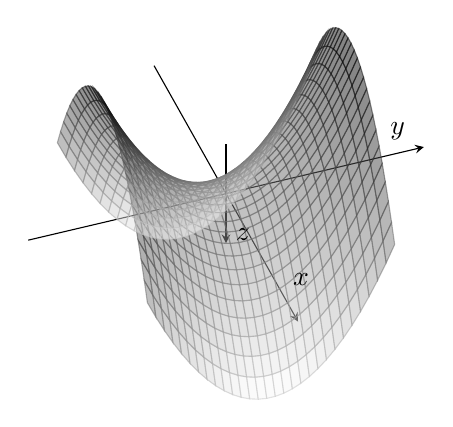
\begin{tikzpicture}
    \begin{axis}[
      xlabel=$x$,
      ylabel=$y$,
      zlabel=$z$,
      view={70}{110},
      axis lines=center,
      xmin=-4, xmax=4,
      ymin=-4, ymax=4,
      zmin=-4, zmax=4,
      ticks=none,
      enlargelimits=0.3,
      clip=false,
    ]

    % Plot the graph of the function with opacity
    \addplot3[
      surf,
      colormap={blackwhite}{gray(0cm)=(0); gray(1cm)=(1)},
      samples=30,
      domain=-4:4,
      y domain=-4:4,
      opacity=0.5,  % Add opacity to the surface
    ]
    {x^2 - y^2};

    % Plot the intersection of the hyperbola with z=4
    \addplot3[domain=-2:2, samples=500, samples y=0, red] ({x}, {sqrt(x^2 - 4)}, {0});
    \addplot3[domain=-2:2, samples=500, samples y=0, red] ({x}, {-sqrt(x^2 - 4)}, {0});

    

    \end{axis}
  \end{tikzpicture}

\begin{tikzpicture} \begin{axis}[
    title={$x^2-x\,y$},
    enlarge x limits,
    view={0}{90},
    xlabel=$x$, ylabel=$y$,
    small,
]
\addplot3[domain=-3:3,
        domain y=-3:3,
        contour gnuplot={levels={-1,1},labels=false},
        thick,samples=50,samples y=50,
    ] {x^2-x*y};
\end{axis}
\end{tikzpicture}

\end{center}




\end{example}
\end{comment}

\newpage


\subsection{Funções de três variáveis: Superfícies de nível}

No caso de funções de três variáveis \( f(x, y, z) \), o conjunto de nível \( N_c \) para um valor constante \( c \) é o conjunto de todos os pontos \((x, y, z)\) no domínio da função para os quais \( f(x, y, z) = c \). Matematicamente, podemos escrever \( N_c = \{(x, y, z) \in \mathbb{R}^3 \mid f(x, y, z) = c\} \).
Geometricamente, a interseção entre $\Gr(f)\subset\R^2$ e hiperplanos em $\R^4$ são superfícies em $\R^3$. 




\begin{example}{}{}
Superfícies de nível da função \(f(x, y, z) = x^2 + y^2 + z^2\) para diferentes valores de \(c\):

\begin{itemize}[label=\color{examplescolor!140}\textbullet]
\item \(c = 0\): Temos 
\[
x^2 + y^2 + z^2 = 0
\]
Neste caso, a superfície de nível é apenas o ponto \((0, 0, 0)\) no espaço tridimensional.


\item\(c > 0\): Para valores positivos de \(c\) temos
\[
x^2 + y^2 + z^2 = c,
\]
ou seja, as superfícies de nível são esferas de raio \(\sqrt{c}\) centrada na origem \((0, 0, 0)\).


\item \(c < 0\): Para valores negativos de \(c\), não existem soluções reais, portanto, não há superfícies de nível pois 
\[
x^2 + y^2 + z^2 = c
\]
não tem nenhuma solução
\end{itemize}


\end{example}


